\subsection{Ranking choice across source representations}\label{sec:sourcefamily}
We tested whether the benefit of restricting candidates changes with the source representation. We held the scene, camera sequence and retained fraction fixed, and compared C with U within each source. We used ordinary 4DGS checkpoints whose saved training configurations disabled prefix supervision. In addition to Chicken, Cut and Sear, we included all five additional real scenes with both an ordinary seed-zero checkpoint and a prefix-supervised source in the prepared-scene archive. These scenes had previously been examined under a different selection protocol. All low-budget comparisons used the same 50\% candidate pool and the same 32 training observations within scene. The comparison addresses transfer between existing sources. Training configurations and final point counts also differ between source families.
\begin{table}[!htbp]\centering\small
\caption{Effect of restricting the influence ranking to the more opaque half of the source. Entries give cold C minus U in mean test PSNR (dB). Both families use seed zero. Each difference compares equal point counts and identical frames within a trained source.}\label{tab:sourcefilter}
\begin{tabular}{lrrrr}\toprule
&\multicolumn{2}{c}{Prefix-supervised}&\multicolumn{2}{c}{Ordinary 4DGS}\\
Scene & 10\% & 15\% & 10\% & 15\% \\\midrule
Chicken & +0.528 & +0.074 & -1.742 & -2.830 \\
Cut Roasted Beef & +1.144 & +0.462 & -0.356 & -0.270 \\
Sear Steak & +0.923 & +0.386 & -0.191 & -0.101 \\
Coffee Martini & +1.092 & +0.521 & -0.356 & -0.720 \\
Flame Steak & +0.618 & +0.290 & -0.001 & -0.187 \\
Broom & +0.577 & +0.179 & -5.820 & -6.973 \\
3Dprinter & +0.120 & +0.032 & -1.966 & -2.937 \\
Peel Banana & +0.387 & +0.080 & -0.683 & -0.982 \\
\bottomrule\end{tabular}\end{table}
Across the eight paired seed-zero scenes in Table~\ref{tab:sourcefilter}, C exceeded U on every prefix-supervised source at both budgets. On ordinary Broom, restricting the candidate pool reduced PSNR by 5.820 and 6.973~dB at 10\% and 15\%, respectively. Appendix~\ref{sec:absolute} gives the native full counts and absolute full, O, C and U PSNR for every pair. U led on all eight ordinary sources at both budgets, with a near tie on Flame Steak at 10\%. On the ordinary Cut source at 10\%, U and C still exceeded opacity by 10.309 and 9.952~dB, respectively. The influence score remains useful on this source even though the filter reduces its benefit.


\runinheading{3}{Independent ordinary training runs.}
We repeated the comparison on three scenes selected from Table~\ref{tab:sourcefilter} to span different seed-zero gaps at 10\%: Broom (largest), Chicken (intermediate) and Flame Steak (smallest). These are within-scene training repeats. We evaluated an existing second Broom checkpoint and trained Chicken and Flame Steak from initialization with a second seed. Each run used the original ordinary scene configuration, 3,000 coarse and 30,000 fine updates, with prefix supervision disabled. The seed pairs shared prepared data, 32 training-only calibration observations, held-out frames and budget rules. Each checkpoint was evaluated at its own native count and at both fixed fractions. Table~\ref{tab:ordrep} gives individual paired effects; the public archive gives absolute full/O/C/U values and individual frame measurements.

\begin{table}[!htbp]\centering\small
\caption{Ordinary 4DGS training repeats. Each cell is U minus C in mean held-out frame PSNR (dB) for one independently trained checkpoint. Both orders retain exactly the same number of primitives within a cell.}\label{tab:ordrep}
\begin{tabular}{lrrrr}\toprule
 & \multicolumn{2}{c}{10\% retention} & \multicolumn{2}{c}{15\% retention}\\
Scene & Seed 0 & Seed 1 & Seed 0 & Seed 1 \\\midrule
Broom & +5.820 & +4.211 & +6.973 & +4.923 \\
Chicken & +1.742 & +2.097 & +2.830 & +3.351 \\
Flame Steak & +0.001 & +0.770 & +0.187 & +1.072 \\
\bottomrule\end{tabular}\end{table}
For the second ordinary Broom, Chicken and Flame Steak sources, U minus C was +4.211, +2.097 and +0.770~dB at 10\% retention, respectively. At 15\%, the corresponding differences were +4.923, +3.351 and +1.072~dB.

Figure~\ref{fig:broom10} shows where the loss occurs on a held-out frame. C breaks up the continuous pavement around the broom and introduces high-contrast streaks across the ground. U recovers the pavement boundary and broom silhouette, although the bristles and fine pavement texture remain softer than the reference. The whole-frame PSNR is 12.74~dB for C, 19.06~dB for U and 23.11~dB for the full source.
\begin{figure}[!htbp]\centering
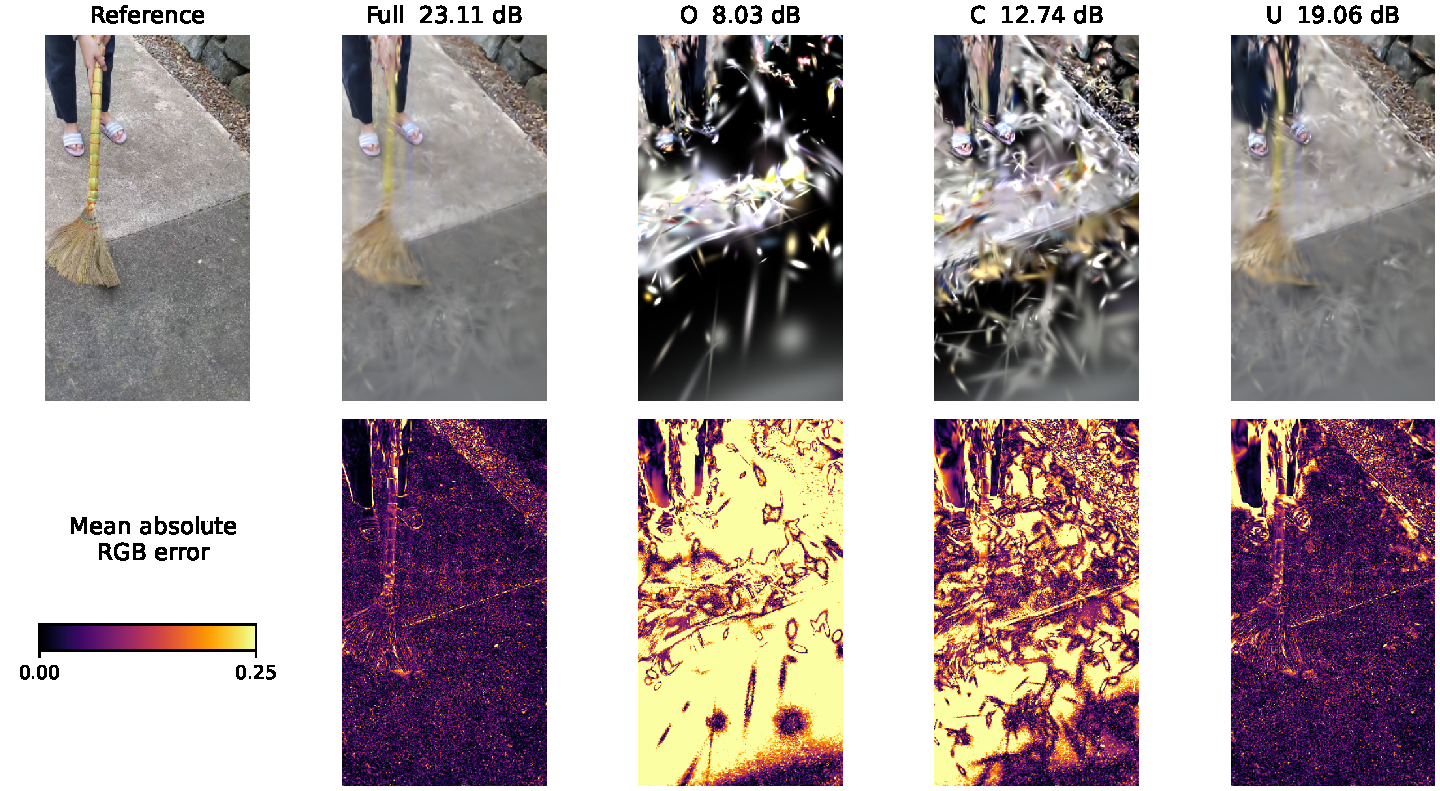
\includegraphics[width=\linewidth]{broom_10.pdf}
\caption{Ordinary Broom at 10\% retention (seed zero, 7,886 of 78,863 points). From left to right: reference image, full source, opacity (O), restricted influence (C) and unrestricted influence (U). Each label is whole-frame PSNR against the reference. The lower row shows mean absolute RGB error on the same linear scale, clipped at 0.25 on $[0,1]$ images. We chose the middle of the 197 held-out frames by list position (zero-based index 98), independently of frame quality.}\label{fig:broom10}\end{figure}

